%********************新章开始*******************************%
\chapter{UBI镜像调试与制作}
\section{UBI镜像在ubuntu中调试优点}
编译出来的需要烧录到模块的ubi镜像是可以放在ubuntu下面进行挂载调试,可以直接利用PC操作模块的文件系统,其优点如下:
\begin{itemize}
  \item PC机的高性能有助于开发人员快速搜索分析ubifs镜像中的可执行文件,配置文件,脚本文件等
  \item 对于配置文件与脚本文件可以直接修改,重新打包下载到模块中
  \item 可以直接确定ubi镜像是否包含修改后代码的编译结果
\end{itemize}
UBI镜像在ubuntu上的调试与制作只需要进行如下工具安装:

\begin{mdframed}[backgroundcolor=lightgray,hidealllines=true]
\begin{verbatim}

darren@darren:~$sudo apt-get install mtd-untils

\end{verbatim}
\end{mdframed}

\section{ubi文件结构主要参数分析}
在挂载ubi文件系统之前,首先要清楚它的几个参数,PEB( Physical Erase Block ),LEB( Logical Erase Blcok ),Page Size,下面是分析linux rootfs的过程:
\begin{mdframed}[backgroundcolor=lightgray,hidealllines=true]
\begin{verbatim}

darren@darren:~$ hexdump -C mdm-perf-recovery-image-mdm9607-perf.ubi | grep "UBI#"
00000000  55 42 49 23 01 00 00 00  00 00 00 00 00 00 00 00  |UBI#............|
00040000  55 42 49 23 01 00 00 00  00 00 00 00 00 00 00 00  |UBI#............|
00080000  55 42 49 23 01 00 00 00  00 00 00 00 00 00 00 00  |UBI#............|
000c0000  55 42 49 23 01 00 00 00  00 00 00 00 00 00 00 00  |UBI#............|
00100000  55 42 49 23 01 00 00 00  00 00 00 00 00 00 00 00  |UBI#............|
00140000  55 42 49 23 01 00 00 00  00 00 00 00 00 00 00 00  |UBI#............|
00180000  55 42 49 23 01 00 00 00  00 00 00 00 00 00 00 00  |UBI#............|

\end{verbatim}
\end{mdframed}

"UBI\#"是struct ubi\_ec\_hdr的魔数,这里的魔数可以简单的理解为标识一个PEB的开始,这里的魔数值可在内核代码中查到,由上可得\wordred{PEB SIZE = 0x0004,0000 - 0x0000,0000 = 256KB}
\begin{mdframed}[backgroundcolor=lightgray,hidealllines=true]
\begin{verbatim}

darren@darren:~$ hexdump -C mdm-perf-recovery-image-mdm9607-perf.ubi | grep "UBI!"
00001000  55 42 49 21 01 01 00 05  7f ff ef ff 00 00 00 00  |UBI!............|
00041000  55 42 49 21 01 01 00 05  7f ff ef ff 00 00 00 01  |UBI!............|
00081000  55 42 49 21 01 01 00 00  00 00 00 00 00 00 00 00  |UBI!............|
000c1000  55 42 49 21 01 01 00 00  00 00 00 00 00 00 00 01  |UBI!............|
00101000  55 42 49 21 01 01 00 00  00 00 00 00 00 00 00 02  |UBI!............|
00141000  55 42 49 21 01 01 00 00  00 00 00 00 00 00 00 03  |UBI!............|
00181000  55 42 49 21 01 01 00 00  00 00 00 00 00 00 00 04  |UBI!............|

\end{verbatim}
\end{mdframed}

"UBI!"是struct ubi\_vid\_hdr的魔数,ubi\_vid\_hdr是标识一个已经分配到ubi卷中的PEB,它与struct ubi\_ec\_hdr各占PEB的前两页中的一页,\wordred{Page SIZE = 0x0000,1000 - 0x0000,0000 = 4KB}

LEB的大小是PEB减去所有头部后剩下的空间,PEB的所头部就是struct ubi\_vid\_hdr与struct ubi\_ec\_hdr,因此,\wordred{LEB SIZE = PEB SIZE - 2*Page SIZE = 248KB}

\section{虚拟MTD设备并挂载ubifs}
正常情况下,我们的ubi镜像是根据flash的参数来确定PEB,LEB,Page SIZE的,但是现在ubi已经做好,所以我们需要根据ubi参数反向推导出flash参数,flash采用的是MTD驱动架构。目前市场上大部份flash都是遵守ONFI( Open Nand Flash Interface )标准,这个标准是由英特尔,闪迪,索尼等多家flash厂商联合制定的,在这份标准中规定,寄存器90H是flash的ID寄存器,这个寄存器包含5个字节的数据。而90H的第四个字节决定了flash的Page SIZE,block SIZE等参数

\begin{figure}[htbp]
\centering
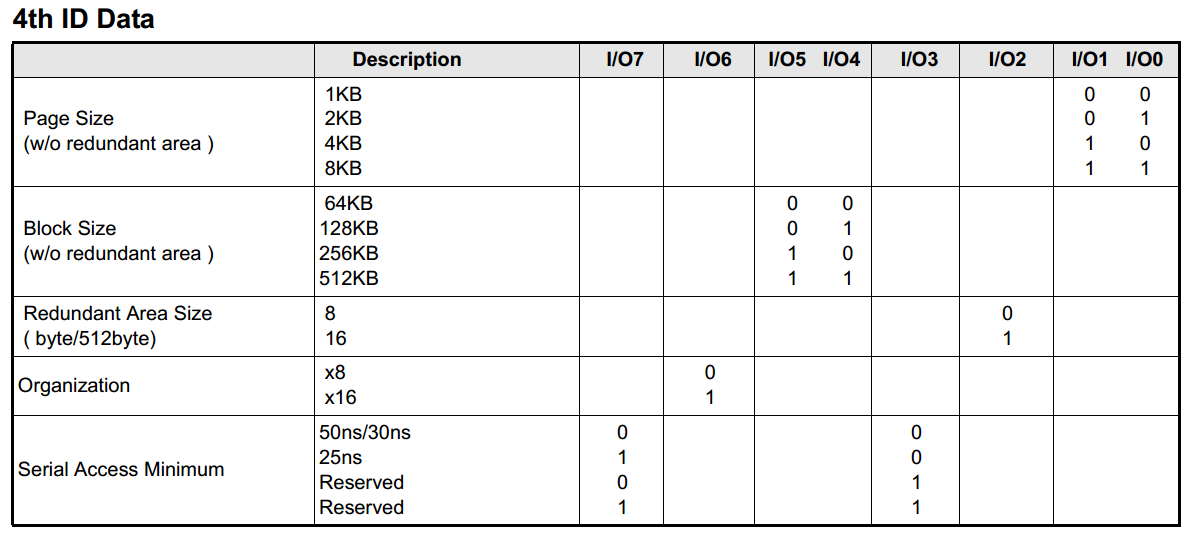
\includegraphics[keepaspectratio,width=\textwidth,height=0.75\textheight]{img/20170517170203.png}
\end{figure}
根据上图获取的信息,就可以使用modprobe nandsim在ubuntu上模拟一个MTD设备了,nandsim的fourth\_id\_byte是我们关注的参数,其它参数可以从ONFI文档中获取
\begin{mdframed}[backgroundcolor=lightgray,hidealllines=true]
\begin{verbatim}

darren@darren:~$ sudo modprobe nandsim first_id_byte=0xec second_id_byte=0xd3
third_id_byte=0x10 fourth_id_byte=0xa6
darren@darren:~$ mtdinfo /dev/mtd0
mtd0
Name:                           NAND simulator partition 0
Type:                           nand
Eraseblock size:                262144 bytes, 256.0 KiB
Amount of eraseblocks:          4096 (1073741824 bytes, 1024.0 MiB)
Minimum input/output unit size: 4096 bytes
Sub-page size:                  1024 bytes
OOB size:                       128 bytes
Character device major/minor:   90:0
Bad blocks are allowed:         true
Device is writable:             true

\end{verbatim}
\end{mdframed}
安装ubi模块,并利用uevent生成/dev/ubi\_ctrl设备节点
\begin{mdframed}[backgroundcolor=lightgray,hidealllines=true]
\begin{verbatim}

darren@darren:~$ sudo modprobe ubi
darren@darren:~$ sudo su
root@darren:~$ echo "add" > /sys/devices/virtual/misc/ubi_ctrl/uevent

\end{verbatim}
\end{mdframed}
将ubi镜像刷入虚拟MTD分区中
\begin{mdframed}[backgroundcolor=lightgray,hidealllines=true]
\begin{verbatim}

darren@darren:~$ sudo ubiformat /dev/mtd0 -f mdm9607-perf-sysfs.ubi -O 4096

\end{verbatim}
\end{mdframed}
注意:这里加-O 4096的目的是让struct ubi\_vid\_hdr所处的位置是一个PEB开始的4096偏移处,如果不这样做,那么struct ubi\_vid\_hdr会处于一个Sub-page size大小的偏移处。如果Sub-page size就是4096,那么就没必要加-O选项了。
\vspace{12 pt}

\noindent 建立MTD设备与ubi联系,并挂载ubi文件系统
\begin{mdframed}[backgroundcolor=lightgray,hidealllines=true]
\begin{verbatim}

darren@darren:~$ sudo ubiattach -m 0 -O 4096
UBI device number 0, total 4096 LEBs (1040187392 bytes, 992.0 MiB), available 0 LEBs (0 bytes), 
LEB size 253952 bytes (248.0 KiB)
darren@darren:~$ mkdir rootfs usrfs
darren@darren:~$ sudo mount -t ubifs /dev/ubi0_0 rootfs/
darren@darren:~$ sudo mount -t ubifs /dev/ubi0_1 usrfs/

\end{verbatim}
\end{mdframed}
至此,ubifs已经成功挂载到ubuntu上了,可以对ubi镜像进行内容搜索,文件修改等操作

\section{反向制作ubi镜像}
制作ubi镜像主要用到两个工具,mkfs.ubifs与ubinize。mkfs.ubifs产生的是ubifs,其中是没有卷标信息的,是不能直接烧写到flash上,但可以通过bootloader中的ubi write函数进行烧写。ubinize产生的是完整的ubi镜像,可以直接烧到flash上进行挂载操作。
\begin{mdframed}[backgroundcolor=lightgray,hidealllines=true]
\begin{verbatim}

darren@darren:~$ mkfs.ubifs -m 4096 -e 253952  -c 2146 -r rootfs/ -F -o rootfs.ubifs
darren@darren:~$ mkfs.ubifs -m 4096 -e 253952  -c 2146 -r usrfs/ -F -o usrfs.ubifs
darren@darren:~$ mkfs.ubifs --help
Usage: mkfs.ubifs [OPTIONS] target
Make a UBIFS file system image from an existing directory tree
Options:
-r, -d, --root=DIR      build file system from directory DIR
-m, --min-io-size=SIZE  minimum I/O unit size(page size)
-e, --leb-size=SIZE     logical erase block size(LEB大小)
-c, --max-leb-cnt=COUNT maximum logical erase block count(只要不比最大容量小就可以)

\end{verbatim}
\end{mdframed}
ubi文件系统做好后,就可以利用ubinize来进行ubi镜像制作。这里要注意,有些ubi镜像包含多个卷,那么每个\wordred{需要内容的卷}都是需要用mkfs.ubifs进行文件系统制作。不需要内容的卷可以直接使用ubinize创建新卷(例如下边的cache卷就是不需要内容的卷)。使用ubinize时,需要一个配置文件,这里写了一个配置文件ubinize.ini
\begin{mdframed}[backgroundcolor=lightgray,hidealllines=true]
\begin{verbatim}

darren@darren:~$ cat ubinize.ini
[sysfs_volume]
mode=ubi
image=rootfs.ubifs
vol_id=0
vol_type=dynamic
vol_name=rootfs
vol_size=63MiB
[usrfs_volume]
mode=ubi
image=usrfs.ubifs
vol_id=1
vol_type=dynamic
vol_name=usrfs
vol_flags = autoresize
[cache_volume]
mode=ubi
vol_id=2
vol_type=dynamic
vol_name=cachefs
vol_size=55MiB
darren@darren:~$ sudo ubinize -o system.ubi -p 256KiB -m 4096 -s 4096 ubinize.ini
darren@darren:~$ ubinize --help
ubinize version 1.5.0 - a tool to generate UBI images. An UBI image may contain one 
or more UBI volumes which have to be defined in the input configuration ini-file
Options:
-o, --output=<file name>    output file name
-p, --peb-size=<bytes>      size of the physical eraseblock of the flash(Kib,Mib可以使用)
-m, --min-io-size=<bytes>   minimum input/output unit size of the flash in byte
-s, --sub-page-size=<bytes> minimum input/output unit used for UBI headers(ubi头部偏移)

\end{verbatim}
\end{mdframed}
至此反向制作的镜像就完成了,system.ubi可以使用前面的方法挂载到ubuntu中使用,也可以直接烧写到模块中进行验证。
\section{删除虚拟MTD设备}
虚拟的MTD设备就是一个nandsim模块,卸载这个模块就行了,在卸载之前,需要把所有挂载在它上面的ubi文件系统umount掉,然后把它与ubi的连接断开
\begin{mdframed}[backgroundcolor=lightgray,hidealllines=true]
\begin{verbatim}

darren@darren:~$ sudo umount rootfs/ usrfs/
darren@darren:~$ sudo ubidetach -m 0
darren@darren:~$ sudo rmmod nandsim

\end{verbatim}
\end{mdframed}
这里,扫尾工作也已经完成。上述过程虽然比较繁琐,但是可以利用脚本来操作,使挂载,制作,卸载等一键完成
